%!TEX root = /Users/Ken/Work/Projects/LesHouches2017/STXSvsEFT/repo/LHStxsVsEft/Documentation/STXSvsSpecificEFTAna.tex
We build a set of gradient BDT classifiers to efficiently discriminate
between the different event hypotheses involved in the analysis, namely $Z b\bar{b}$,
SM $Z H$, and BSM $Z H$ production. 
The classifiers receive kinematic variables related to the event as inputs and approximate
the likelihood for each event to belong to any of the three classes.

\begin{equation}
p_{i}(\vec x) = \frac{ e^{\beta_{i}(\vec x) } }{ \sum_j e^{\beta_{j}(\vec x) } }
\end{equation}
here $\vec x$ represents all the input variables to the discriminant, that are shown in Table~\ref{tab:bdt_features} \red{(Definition of $\beta_i$)}.

These kind of algorithms are regularly used by the experimental analyses and often provide a comparable performance to those of more sophisticated techniques such as matrix element methods. 
%
\begin{table}[h!]
\centering
\begin{tabular}{||c|c||c|c||}
variable definition & variable name &  variable name & variable definition \\
\hline
$p_T(l_1)$ & leading lepton $p_T$ & $p_T(l_2)$ & sub-leading lepton $p_T$\\
$p_T(b_1)$ & leading b-jet $p_T$ & $p_T(b_2)$ & sub-leading b-jet $p_T$\\
$\eta(l_1)$ & leading lepton pseudo-rapidity & $\eta(l_2)$ & sub-leading lepton pseudo-rapidity\\
$\eta(b_1)$ & leading b-jet pseudo-rapidity  & $\eta(b_2)$ & sub-leading b-jet  pseudo-rapidity\\
$y(Z)$ & Z-candidate rapidity  & $y(H)$ & H-candidate rapidity \\
$p_T(Z)$ & Z-candidate $p_T$  & $m_{bb}$ & H-candidate invariant mass \\
$m_{VH}$ & HZ invariant mass  &  &  \\
\end{tabular}
\caption{
\label{tab:bdt_features}
Input variables used by the kinematic BDT discriminants.
}
\end{table}

Five sets of discriminants were trained:
\begin{enumerate}
\item A binary discriminant to separate $Z b\bar{b}$ production from the SM $Z H$ production.
\item Four sets of \red{three(/multi?)-class} discriminants (one for each of the $c_{\sss HW}$ benchmarks) to
    discriminate between $Z b\bar{b}$, SM $Z H$ and BSM $Z H$ production.
\end{enumerate}
The first discriminant was used to reduce the $Z b\bar{b}$ background in the template
cross section analysis, in such a way to mimic the experimental analyses.
The last four discriminants were used to first reduce the $Z b\bar{b}$ background and then to further classify the selected events to discriminate between the SM and BSM hypotheses.

The BDTs were trained using the scikit-learn~\cite{scikit-learn} and xgboost packages~\cite{xgboost}. To this end, the events were
split into two statistically independent samples, with a ratio of 3:1, used respectively for training and
application of the discriminants. % Three quarters of the events were used for training.
We used the categorical cross-entropy loss function, and the algorithm hyperparameters were
optimised on the training sample using stochastic grid search and the mean
k-fold cross-validation loss as figure of merit, with $k = 5$.
The optimized hyperparameters are shown in Table~\ref{tab:bdt_hpars}.

\begin{table}
\centering
\begin{tabular}{||c|c||}
parameter & value \\
\hline
number of trees & 600 \\
maximum depth & 5 \\
bagging fraction & 0.8 \\
learning rate & 0.05 \\
$L_2$ regularisation strength & 1 \\
\end{tabular}
\caption{
\label{tab:bdt_hpars}
Optimized BDT training hyperparameters.
}
\end{table}

After training, the $p(Z b\bar{b})$ variables were used to define selection criteria
for the events to be considered for analysis. The maximum allowed value for $p(Z b\bar{b})$
was determined in order to maximise the quantity $\varepsilon^2(SM Z H) / \varepsilon(Z
b\bar{b})$, where $\varepsilon$ is the selection efficiency of a given sample. Such a
figure of merit is, in the gaussian limit, proportional to the squared median expected
discovery significance to observe the standard model production of of $Z H$.
The choice was made again to mimic the experimental analyses, for which the observation of
the SM Higgs signal will be the primary goal.

In order to ensure a smooth behaviour, the figure $\varepsilon^2(SM Z H) /
\varepsilon(Zb\bar{b})$ was regularised by replacing $\varepsilon(Zb\bar{b})$ with
$\varepsilon(Zb\bar{b}) \oplus \varepsilon_0$ where $\oplus$ denotes the sum in quadrature
and $\varepsilon_0 = 0.03$.
Figure~\ref{fig:s2_over_b} shows, as an example, the result of the optimisation scan for
the discriminant trained to separate $Z b\bar{b}$ production from the SM $Z H$
production. The analysis was repeated separately for each of the 5 discriminants and
similar results were obtained in all cases.

\begin{figure}
\centering
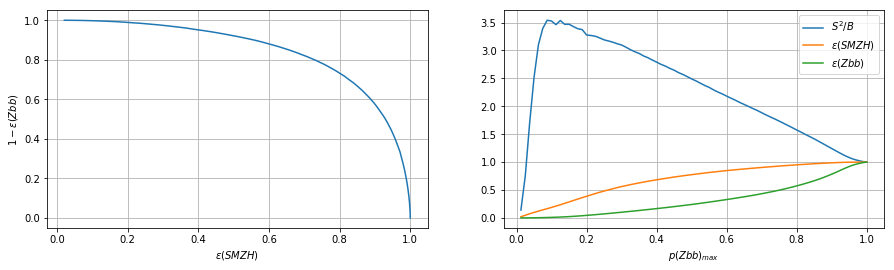
\includegraphics[width=0.8\textwidth]{plots/bkg_cut_opt.png}
\caption{
\label{fig:s2_over_b}
Optimisation analysis to determine the maximum value of $p(Z b\bar{b})$ for events
considered in the analysis. (left) {\it ROC} curve for $Z b\bar{b}$ vs SM $Z H$
separation. (right) Regularised $\varepsilon^2(SM Z H) /
\varepsilon(Zb\bar{b})$ as a function of the $p(Z b\bar{b})_{max}$.
\red{the plots are a bit pixellated, are there PDF versions available?}
}
\end{figure}

For this exploratory study, we only considered four BSM benchmarks, varying $c_{\sss HW}$ and testing the
sensitivity to each of these benchmarks using a dedicated set of kinematic
discriminants. While the design of an optimal discriminant that continuously depends on
the BSM parameters is beyond the scope of this work, we investigated the degree of
correlation between the BSM discriminants for each of the scenarios.
Figure~\ref{fig:bdt_corr} shows the linear correlation coefficient between $p(BSM)$ for
each of the four scenarios, evaluated on SM $Z H$ production events \red{(can we add one sentence to qualitatively describe what this measures?)}. As it can be seen,
the linear correlation varies between 0.3 and 0.96, and it increases as the distance
between the benchmark points decreases. This suggests that the information used to
discriminate the different benchmarks is similar, but that optimal results are obtained
when a specific benchmark is targeted.

\red{everything below, inlcuding table, overlaps with the stats analysis sections -- need to decide where to put it}
Finally, we compare the selection efficiency of selecting events according to the $p(Z
b\bar{b})$ discriminant trained to separate $Z b\bar{b}$ production from the SM $Z H$
production. \red{QUESTION: What are the BDT cuts used?} A difference in these figures would directly affect any analysis based on STXS that are extrapolated to a larger phase space assuming SM $Z
H$ kinematics. As can be seen in Table~\ref{tab:bdt_efficiency}, relative differences in efficiencies of the order of 20-50\% are observed. \red{In general, the sensitivity to any non-SM contribution to a measured cross section can only come from the events recorded in the fiducial volume, prior to any model-dependent extrapolations.}
%
% \blindtext

\newfloatcommand{capbtabbox}{table}[][\FBwidth]
\begin{figure}[h!]
\begin{floatrow}
\ffigbox{%
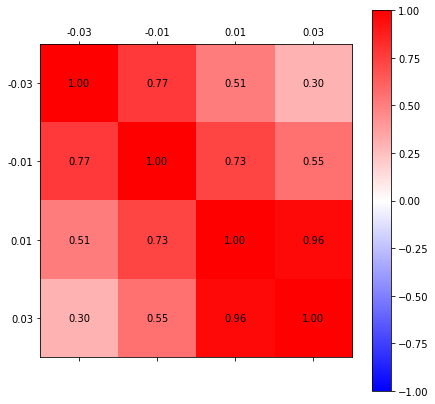
\includegraphics[width=0.8\linewidth]{plots/bdt_corr.png}
}{%
  \caption{\label{fig:bdt_corr}A figure
  Linear correlation coefficient between $p(BSM)$ for
  each of the four scenarios, evaluated on SM $Z H$ production events.
  Row and columns are labelled by the value of $c_{\sss HW}$.
  }%
}
\hspace{1cm}
\capbtabbox{%
\hspace{1cm}
\begin{tabular}{||c|c||}
sample & $\varepsilon$  \\
\hline
$c_{\sss HW} = 0.03$ & 0.14 \\
$c_{\sss HW} = 0.01$ & 0.16 \\
SM & 0.19 \\
$c_{\sss HW} = -0.01$ & 0.23 \\
$c_{\sss HW} = -0.03$ & 0.32 \\
\end{tabular}
\hspace{1cm}
\vspace{1.2cm}
}{%
  \caption{
  \label{tab:bdt_efficiency}
  Selection efficiency for the $p(Z b\bar{b})$ selection for different scenarios. The
  efficiency is computed for events in the fiducial volume defined in Table~\ref{tab:FiducialXS}.
  \red{can we add the efficiency for Zbb to show how well it rejects and also use the number later in the text?}
  }%
}
\end{floatrow}
\end{figure}

% \end{document}
% \begin{figure}[h!]
% \centering
% 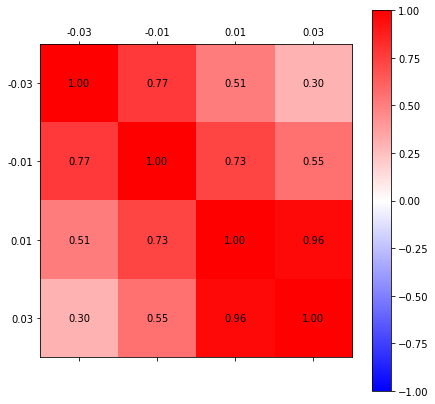
\includegraphics[width=\linewidth]{plots/bdt_corr.png}
% \caption{
% \label{fig:bdt_corr}
% Linear correlation coefficient between $p(BSM)$ for
% each of the four scenarios, evaluated on SM $Z H$ production events.
% Row and columns are labelled by the value of $c_{\sss HW}$.
% }
% \end{figure}
%
% \begin{table}
% \centering
% \begin{tabular}{||c|c||}
% sample & $\varepsilon$  \\
% \hline
% $c_{\sss HW} = 0.03$ & 0.14 \\
% $c_{\sss HW} = 0.01$ & 0.16 \\
% SM & 0.19 \\
% $c_{\sss HW} = -0.01$ & 0.23 \\
% $c_{\sss HW} = -0.03$ & 0.32 \\
% \end{tabular}
% \caption{
% \label{tab:bdt_efficiency}
% Selection efficiency for the $p(Z b\bar{b})$ selection for different scenarios. The
% efficiency is computed for events in the fiducial volume defined in Table~\ref{tab:FiducialXS}.
% }
% \end{table}
%
%

%%% Local Variables:
%%% mode: latex
%%% TeX-master: "STXSvsSpecificEFTAna"
%%% End:
